Her har det vært mye uklarheter.


Vi er blitt fortalt at det norske ordet
for universal bias er spenningsfordeler.
Etter å ha sett på flere kilder ser det ut til at
spenningsfordeling er noe som skjer, og må tas hensyn til,
under universal bias stabilization.

Formålet med universal bias stabilization, er å få et
stabilt Q-punkt (forklart straks).
Dette er bra for å få en gjevn $I_C$ uavhengig av $\beta$.

\subsubsection{Lastlinje}
Lastlinjen viser alle \emph{mulige} kombinasjoner av $I_C$ og $V_{CE}$.

For å ta hensyn til temperaturforandringer og andre forstyrrelser,
velger vi et punkt midt på denne linja.
\\\\
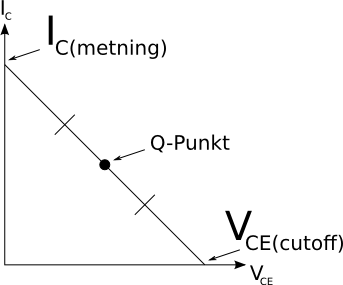
\includegraphics[width=0.5\textwidth]{./img/lastlinje}
\\\\
$$I_{C(metning)} = \frac{V_{CC}}{R_C}$$
$$V_{CE(cutoff)} = V_{cc}$$
Man bruker dette når man velger hvor store motstandere man vil ha.
$$R_C = \frac{V_{CE}}{I_C}$$

